\documentclass[a4paper,10pt]{article}
\usepackage[ngerman]{babel}
\usepackage[utf8]{inputenc}
\usepackage[a4paper,vmargin={20mm,20mm},hmargin={20mm,10mm}]{geometry}
\usepackage[T1]{fontenc}

\usepackage{tocloft, multicol} 
\usepackage{amsmath, amsfonts, amssymb} 
\usepackage{booktabs} 
\usepackage{bm}  
\usepackage{caption}
\usepackage{subcaption}
\usepackage{enumitem}
\usepackage{graphicx} 
\usepackage{listings}
\usepackage{mathtools}
\usepackage[dvipsnames]{xcolor}
\usepackage{wrapfig,lipsum,threeparttable}
\usepackage{footmisc, fixfoot}



\DeclareFixedFootnote{\fnrefa}{ P. T. Boggs and J. E. Rogers, “Orthogonal Distance Regression,” in “Statistical analysis of measurement error models and applications: proceedings of the AMS-IMS-SIAM joint summer research conference held June 10-16, 1989,” Contemporary Mathematics, vol. 112, pg. 186, 1990. }
\DeclareFixedFootnote{\fnrefb}{ Dr. J.Wagner - Physikalisches Anfängerpraktikum - V. 1.1 Stand 1/2018, Versuch 213}
\DeclareFixedFootnote{\fnrefc}{ Dr. J.Wagner - Physikalisches Anfängerpraktikum - V. 1.2 Stand 06/2016, Versuch 14}

\lstset{literate=%
    {Ö}{{\"O}}1
    {Ä}{{\"A}}1
    {Ü}{{\"U}}1
    {ß}{{\ss}}1
    {ü}{{\"u}}1
    {ä}{{\"a}}1
    {ö}{{\"o}}1
    {~}{{\textasciitilde}}1
}
\lstset{%
backgroundcolor=\color{gray!32},
basicstyle=\ttfamily\footnotesize,
numbers=left,numberstyle=\scriptsize,
frame=single,
breaklines=true,
}


\usepackage[wby]{callouts}
\title{WS19/20, PAP2.1, Versuch 213:\\ Kreisel}
\date{Versuchsdurchführung: \\22. Oktober, 2019}
\author{Praktikanten:\\Gerasimov, V. \& Reiter, L.\\\\ Betreuer:\\ Neitzel, C.}


\begin{document}

\maketitle

\newpage

\tableofcontents

\addtocontents{toc}{~\hfill\textbf{Seite}\par}

\section[Einführung]{Einführung\fnrefb}\boldmath
Dieser Versuch befasst sich mit den grundlegenden physikalischen Eigenschaften von Kreiseln und ihrer Vermessung.
Zuerst wollen wir in einem Vorversuch qualitativ das Verhalten eines Kreisels untersuchen. Danach messen wir die Reibungsverluste des Kreisels und bestimmen die Dämpfungskonstante \(k\) und Halbwertszeit \(T_{1/2}\). Wir bestimmen aus der Präzessionsfrequenz eines schweren Kreisels sein
Trägheitsmoment \(I_{z}\) um die Figurenachse \(\vec{Z}\). Das Trägheitsmoment \(I_{x}\) senkrecht zur Figurenachse bestimmt wir aus der Größe und der Richtung der Umlaufsgeschwindigkeit  \(\Omega\) der momentanen Drehachse um die Figurenachse des Kreisels und zusätlich ein zweites Mal aus der gemessenen Nutationsfrequenz  \(f_{N}\).

\begin{itemize}
\item Ein starrer Körper, der um einen festen Punkt rotiert, stellt einen Kreisel dar. Sind genau zwei Hauptträgheitsmomente identisch \((I_{x}=I_{y})\), so wird der Kreisel als symmetrisch bezeichnet. Wird der Kreisel im Schwerpunkt unterstützt so heißt der Kreisel kräftefrei. In diesem Fall wirken keine äußeren Drehmomente und der Drehimpuls ist räumlich und zeitlich konstant.

\item Die allgemeine Bewegung eines kräftefreien Kreisels stellt eine Nutationsbewegung dar. Dabei fuhrt die Figurenachse eine Eigendrehung mit \(\omega_F\) durch und rotiert mit der Nutationsfrequenz \(\omega_N\) gleichzeitig um die raumfeste Drehimpulsachse. Die Winkelgeschwindigkeit ist nicht konstant sondern bewegt sich mit \(\Omega\) um die Figurenachse \(\vec{Z}\). Diese Bewegung kann mit Hilfe einer farbigen Sektorscheibe beobachtet werden. Die Bewegungen der charakteristischen Kreiselachsen kann man sich durch ein Abrollen eines körperfesten Kegels auf einen raumfesten Kegels veranschaulichen.

\item Liegt der Auflagepunkt des Kreisels nicht im Schwerpunkt, so heißt der Kreisel schwerer Kreisel. In diesem Fall übt die Gewichtskraft ein Drehmoment aus, das zu einer Präzession führt. Dabei bewegt sich der Drehimpuls mit der Frequenz  \(\omega_P\) auf einem Kegelmantel um die Richtung der Gewichtskraft.


\end{itemize}

\section[Versuchsaufbau, Literaturwerte \& Vorbereitung]{Versuchsaufbau\fnrefb, Literaturwerte \& Vorbereitung}
\begin{itemize}
\item Stahlkugel mit Aluminiumstab (Masse \(m_K = 4.164(1) \: kg\) incl. Stab, Kugelradius \(r_K=5.08(1)\: cm\)) als Kreisel gelagert in einer Luftkissenpfanne
\item 2 Gewichte (\(r_a=0,725(1)\: cm\),  \(r_i=0,325(1)\: cm\),  \(h_G=1,10(1)\: cm\),  \(m_G=9,85(1)\: g\))
\item Farbscheibe, Scheibe mit konzentrischen Ringen
\item Stroboskop, optischer Drehzahlmesser
\item Stoppuhr
\item Motor mit Netzgerät
\item Gyroskop zur Demonstration der Kreiseleigenschaften
\item Literaturwert für Erdbeschleunigung\fnrefc in Heidelberg, Baden Württemberg, Deutschland: \(g=9.80984(2)\:m\:s^2\)
\end{itemize}

\section{Vorversuch: qualitative Beobachtung des Verhaltens eines Kreisels }
\subsection[Durchführung]{Durchführung\fnrefb}
Der Vorversuch soll uns mit dem Kreisel vertraut machen und uns die später genauer zu untersuchenden Erscheinungen qualitativ demonstrieren.
\begin{enumerate}[label=(\alph*)]
\item Wir öffnen das Druckluftventil an der Wand, stecken die Scheibe mit den Farbsektoren nach oben auf den Stab und balancieren die Scheibe wie zuvor beschrieben aus, sodass der Kreisel kräftefrei wird. Der Kreisel wird auf einige Umdrehungen pro Sekunde beschleunigt und wir beobachten die
Reaktion des Kreisels, wenn der Metallring des Kugellagers am Stabende mit einem Finger zur Seite gedrückt wird. Alle Beobachtungen werden erläutert.

\item Als nächstes stellen wir eine Nutationsbewegung ein, indem dem Stab ein leichter, seitlicher Stoß erteilt wird. Die Farbscheibe ist zu beobachten: In der mischfarbigen Fläche der sich drehenden Scheibe soll ein Punkt zu erkennen sein, an dem eine "reine, unvermischte" Farbe erscheint. An dieser Stelle ändert
sich die Farbe gemäß der Farbanordnung auf der Sektorscheibe. Dieser Punkt stellt den um die Figurenachse \(\vec{Z}\) wandernden Ort der momentanen Drehachse \(\vec{\omega}\) dar.\\\\
Wir drehen die Scheibe um, sodass die Seite mit den farbigen Ringen nach oben zeigt und wiederholen den Versuch. Wenn beim Anschlagen des Kreisels einen Nutationskegel erreicht wird, der gerade in einem der Farbringe
verläuft, ändert sich die Farbe am Ort der momentanen Drehachse nicht, d.h.
\(\vec{\omega}\) läuft auf einem Kreis um \(\vec{Z}\).

\item Wir legen zusätzlich die Scheibe mit den konzentrischen Kreisen auf die Farbscheibe und wählen zunächst die Seite der Scheibe, bei der der Mittelpunkt der Kreise seitlich gegen die Aufnahmeachse verschoben ist. Liegt keine Nutation vor \( ({\vec{\omega} || \vec{Z}}) \), so erkennt man ein System konzentrischer, verwaschener Kreise um den Stab. D.h. der Mittelpunkt des Kreissystems zeigt die Drehachse an. Danach drehen wir die Scheibe um und versetzen  den Kreisel in Rotation. Durch einen seitlichen Stoß werden wieder die drei Kreiselachsen getrennt. Warum markiert jetzt der Mittelpunkt der verwaschenen Kreise die Drehimpulsachse, die räumlich stehen bleibt?\\\\
Wir Bringen ein Zusatzgewicht am Stab an und wiederholen den Versuch. Die Drehimpulsachse sollte nun ein Präzessionsbewegung durchführen.

\item Ohne zusätzliche Farbscheibe richtet sich der Stab immer auf, d.h.
der Schwerpunkt liegt unterhalb der Kugelmitte. Mit einem Zusatzgewicht am Ende des Stabes fällt dagegen der Kreisel um. In diesem Fall liegt der Schwerpunkt oberhalb der Kugelmitte. Wir versetzen in beiden Fällen den Kreisel in Drehung, lassen den Stab aus einer nichtvertikalen Stellung los und beobachten die Drehrichtung der Präzession. Danach  wir die Drehrichtung des Kreisels geändert und der Versuch wiederholt.
\end{enumerate}
\subsection{Auswertung}
\begin{enumerate}[label=(\alph*)]
\item Ohne angebrachte Farbscheibe ist der Kreisel in der Luftkissenpfanne zuerst nicht kräftefrei. D.h. es kommt zur Präzession, einer zeitlichen Änderung der Richtung des Drehimpulses und der Figurenachse, weil auf den Kreisel ein äußeres Drehmoment \(\vec{M}\) wirkt.\\\\
Nachdem die Farbscheibe mit den Sektoren angebracht und ausbalanciert wurde, verschwindet das äußere Drehmoment und der nun kräftefreie Kreisel behält seinen Drehimpuls bei (im Falle von vernachlässigbarer Reibung). Die Figurenachse  \(\vec{Z}\) änder sichjetzt nur noch leicht aufgrund der leichten restlichen Nutation.
Der Kreisel behält nach dem Drücken seine Drehachse bei und die Farbsektoren verschwimmen zu einer Mischfarbe. Beim Drücken des Kugellagers spürt man einen deutlichen Widerstand, der mit zunehmender Drehfrequenz des Kreisels auch zunimmt.

\item Nachdem sich die Nutationsbewegung eingestellt hat, lässt sich auf dem Farbsektorenring ein Kreis beobachten, der abwechselnd jeweils eine der 3 ursprünglichen Farben annimmt.\\\\
Wenn die Scheibe mit den Farbringen angebracht wird, so entsteht ein einfarbiger Punkt in der Mitte, der seine Farbe mit der Zeit nicht ändert, aber die Farbe ändert sich für verschiedene Nutationswinkel.

\item Beide Scheiben mit den konzentrischen Kreisen erzeugen unterschiedlich stark verschwommene Ringsysteme die sich zeitlich nicht ändern, aber vom Nutationswinkel abhängen. Ein einfarbiger Punkt in der Mitte zeigt ungefähr in die ursprüngliche Richtung der Drehachse (bevor die Nutation eingeleitet wurde) und die 
Figurenachse \(\vec{Z}\) kreist um ihn  (Nutation). Diese Punkt zeigt uns die Richtung der momentanen Drehachse \(\vec{\omega}\) an.\\\\
Sobald ein Zusatzgewicht am Stab angebracht wird fängt der zuvor räumlich feste einfarbige Punkt an zu wandern. Seine Bewegung entspricht nun der Präzessionsbewegung des Kreisels, da die Figurenachse jetzt eine Kombination aus Nutations- und Präzessionsbewegung vollführt.
\item Ohne Farbscheibe und Zusatzgewichte sind die Richtungen der Eigendrehung und Präzessionsdrehung entgegengesetzt und mit Zusatzgewicht zeigen beide in die gleiche Richtung. Bei Änderung der Eigendrehung in die andere Richtung ändern sich auch Nutations-  und Präzessionsdrehrichtung. Wie erwartet bleiben die Beziehungen zwischen den betrachteten Drehrichtungsvektoren erhalten, wenn alle Vektoren das Vorzeichen ändern.

\end{enumerate}
\section{Messung der Reibungsverluste \& Bestimmung der Dämpfungskonstante und Halbwertszeit}
\subsection[Durchführung]{Durchführung\fnrefb}
Wir bringen wieder die Sektorenscheibe an und überprüfen ob der Kreisel kräftefrei ist. Zusätzlich montieren wir beide Gewichte am Stabende.
Der Kreisel wird mit Hilfe des Motors bei senkrechter Achse auf eine Anfangsfrequenz \(f_{0}\approx600-700\:{min}^{-1}\) beschleunigt.  Alle 2 Minuten wird die Drehfrequenz des Kreisels über einen Zeitraum von 12 Minuten gemessen. Die Drehfrequenz \(f\) zur jeweiligen Zeit \(t\) wird notiert.

\subsection{Messergebnisse}
Messdaten wurden dem Versuchsprotokoll (22. Oktober, 2019) entnommen und in Tabelle \ref{tab:Tab1} übertragen.
\unboldmath
\begin{table}[htb]
\centering
\caption{Messung der Drehfrequenz}\label{tab:Tab1}
\begin{threeparttable}
\begin{tabular}{cc}
\toprule
Zeit \boldmath\(t\)\unboldmath & Drehfrequenz \boldmath\(f\)\unboldmath \\
\([s]\)&\([min^{-1}]\)\\
\midrule
\(0\pm2\)&\(648\pm10\)\\
\(120\pm2\)&\(600\pm10\)\\
\(240\pm2\)&\(552\pm10\)\\
\(360\pm2\)&\(515\pm10\)\\
\(480\pm2\)&\(470\pm10\)\\
\(600\pm2\)&\(437\pm10\)\\
\(720\pm2\)&\(403\pm10\)\\
  \bottomrule
 \end{tabular}
\begin{tablenotes}
\raggedright
\item[1]sowohl \boldmath\(\Delta t \) als auch \(\Delta f \) sind grob abgeschätzt\unboldmath
\end{tablenotes}
\end{threeparttable}\end{table}
\boldmath

\subsection{Kurvenanpassung mit Python}
\subsubsection{Source Code \& Input}
Wir drücken zuerst \(f\) über die entsprechende Kreisfrequenz \(\omega\) aus:
\begin{equation} \label{eq:omega}
	\omega=2\pi f
\end{equation} 
\begin{equation} \label{eq:Deltaomega}
	\Delta\omega=2\pi (\Delta f)
\end{equation} 
Wir gehen davon aus, dass die die Kreisfrequenz exponentiell mit der Zeit abnimmt.
Daher ist unser funktionales Modell für die Ausgleichungsrechnung wie folgt:
\begin{equation} \label{eq:Fit1}
	\boxed{\omega=\omega_{0} e^{-k t}}
\end{equation} 
So sieht unsere Python-Implementierung aus:\\

Header:
\begin{lstlisting}
%matplotlib inline
import matplotlib.pyplot as plt
import numpy as np
from scipy.stats import chi2
from decimal import Decimal

def format_e(n):
    a = '%e' % Decimal(n)
    return a.split('e')[0].rstrip('0').rstrip('.')+'e'+a.split('e')[1]
\end{lstlisting}

Messwerte aus Tabelle \ref{tab:Tab1} in SI Einheiten:
\begin{lstlisting}
t = np.array([0,120,240,360,480,600,720]
Fehler_t = np.array([2,2,2,2,2,2,2])

f = np.array([648,600,552,515,470,437,403]) /60
Fehler_f = np.array([10,10,10,10,10,10,10]) /60

\end{lstlisting}

Berechnung von \(\omega\) und \(\Delta\omega\) nach \eqref{eq:omega} bzw. \eqref{eq:Deltaomega}:\begin{lstlisting}
omega = 2*np.pi*f
Fehler_omega = 2*np.pi*Fehler_f

\end{lstlisting}

Fitfunktion \eqref{eq:Fit1} wird deklariert:\begin{lstlisting}
from scipy import odr

def fit_func(p, x):
    (A, k) = p 
    return A*np.exp(-k*x)

model = odr.Model(fit_func)

\end{lstlisting}

darzustellende Daten werden übergeben:\begin{lstlisting}
x = t
y = omega
delta_x = Fehler_t
delta_y = Fehler_omega

\end{lstlisting}

Startparameter für Ausgleichungsrechnung werden gesetzt, sodass Lösung konvergiert:\begin{lstlisting}
para0 = [1, 0]

data = odr.RealData(x, y, sx=delta_x, sy=delta_y)
odr = odr.ODR(data, model, beta0=para0 )
out = odr.run()

\end{lstlisting}

Endgültige Ausgleichungsparameter und ihre Kovarianzmatrix werden ausgelesen:\begin{lstlisting}
popt = out.beta
perr = out.sd_beta

\end{lstlisting}

Angabe welche Sigma-Umgebung der Fitfunktion im Diagramm dargestellt werden soll:\begin{lstlisting}
nstd = 10

popt_top = popt+nstd*perr
popt_bot = popt-nstd*perr

\end{lstlisting}

Plot-Umgebung wird angegeben:\begin{lstlisting}
x_fit = np.linspace(min(x)-(max(x)-min(x))/10, max(x)+(max(x)-min(x))/10, 1000)
fit = fit_func(popt, x_fit)
fit_top = fit_func(popt_top, x_fit)
fit_bot = fit_func(popt_bot, x_fit)

\end{lstlisting}

Diagramm (Abb.\ref{fig:Fig1}) wird erstellt:\begin{lstlisting}
fig, ax = plt.subplots(1)
plt.ticklabel_format(axis='both', style='sci', scilimits=(0,3), useMathText=True)
plt.errorbar(x, y, yerr=delta_y, xerr=delta_x, lw=1, ecolor='k', fmt='none', capsize=1, label='Messdaten')
plt.title('Kreisfrequenz als Funktion der Zeit')
plt.grid(True)
plt.yscale('log')
plt.xlabel('Zeit '+r'${t}$'+' '+r'${[s]}$')
plt.ylabel('Kreisfrequenz '+r'${\omega}$'+' '+r'${[Hz]}$')
plt.plot(x_fit, fit, 'r', lw=1, label='Fit')
ax.fill_between(x_fit, fit_top, fit_bot, color='C3', alpha=.25, label=str(nstd)+r'$\sigma$'+'-Umgebung')
plt.legend(loc='best')

plt.savefig('figures/213_Fig1.pdf', format='pdf', bbox_inches='tight')

\end{lstlisting}

Der Chi-Quadrat-Test wird durchgeführt unter Berücksichtigung von \( \Delta t\) und \(\Delta \omega\). D.h.~es wird jeweils der senkrechte/orthogonale Abstand der Messwerte zur Fitfunktion (Abb.\ref{fig:chi}) berechnet und normiert\fnrefa.
 Die Summe der normierten Abstandsquadrate, der \unboldmath\( \chi^{2}\)-Wert, wird  reduziert.\boldmath

\begin{figure}[htb]
  \centering
  \begin{annotate}{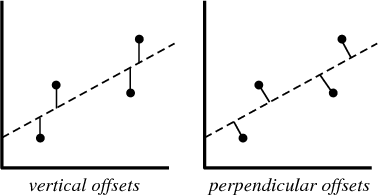
\includegraphics[width=0.5\textwidth]{chi.png}}{1}
  \end{annotate}
\caption[Abstände von Messdaten zur Fitfunktion]{Abstände von Messdaten zur Fitfunktion\footnotemark}
\label{fig:chi}
\end{figure}
\footnotetext{http://mathworld.wolfram.com/LeastSquaresFitting.html}

\begin{lstlisting}
dof = x.size-popt.size
chisquare = out.sum_square
chisquare_red = chisquare/dof
prob = round(1-chi2.cdf(chisquare,dof),2)*100

\end{lstlisting}

Auslesen der Messergebnisse:\begin{lstlisting}
omega_0 = popt[0]
Fehler_omega_0 = perr[0]

k = popt[1]
Fehler_k = perr[1]

\end{lstlisting}

Die Halbwertszeit können wir nun sofort aus der Dämpfungskonstante \(k\) berechnen:
\begin{equation} \label{eq:T_halb}
T_{1/2} = ln(2)/k
\end{equation}
\begin{equation} \label{eq:DeltaT_halb}
\Delta T_{1/2}=|T_{1/2}\left(\frac{\Delta k}{k}\right)|
\end{equation}
Berechnung von \(T_{1/2}\) und \(\Delta T_{1/2}\) nach \eqref{eq:T_halb} bzw. \eqref{eq:DeltaT_halb}:\begin{lstlisting}
T_halb = np.log(2)/k
Fehler_T_halb = T_halb*Fehler_k/k

\end{lstlisting}

Ausgabe der Messergebnisse wird erstellt:\begin{lstlisting}
print('Startwert der Kreisfrequenz: ')
print('omega_0 [Hz] =', format_e(omega_0), ' +- ', format_e(Fehler_omega_0))
print('Chi-Quadrat =', chisquare)
print('Freiheitsgrade =', dof)
print('Chi-Quadrat reduziert =', chisquare_red)
print('Wahrscheinlichkeit ein größeres oder gleiches Chi-Quadrat zu erhalten =', prob, '%')
print('\n')
print('Dämpfungskonstante: ')
print('k [Hz] =',  format_e(k), ' +- ',  format_e(Fehler_k))
print('\n')
print('Halbwertszeit: ')
print('T_halb [s] =',  format_e(T_halb), ' +- ',  format_e(Fehler_T_halb))
\end{lstlisting}
\subsubsection{Output}
\begin{lstlisting}
Startwert der Kreisfrequenz: 
omega_0 [Hz] = 6.791995e+01  +-  1.653924e-01
Chi-Quadrat = 0.2262760874189914
Freiheitsgrade = 5
Chi-Quadrat reduziert = 0.04525521748379828
Wahrscheinlichkeit ein größeres oder gleiches Chi-Quadrat zu erhalten = 100.0 %

Dämpfungskonstante: 
k [Hz] = 6.600142e-04  +-  6.605926e-06

Halbwertszeit: 
T_halb [s] = 1.0502e+03  +-  1.051121e+01
\end{lstlisting}
Wir erfahren also sofort, dass
\begin{align*}
k&=6.600(66)\times10^{-4}\: Hz\\
T_{1/2}&=1.050(11)\times10^{3}\:s
\end{align*}
und als Ergebnis auf unseren Anpassungstest:
\[\chi^{2}_{red}=4.5\times10^{-2}\]
Die Wahrscheinlichkeit ein größeres oder gleiches Chi-Quadrat zu erhalten ist
 \[P\approx  100.0 \%\]
und wir erhalten das Diagramm in Abb.\ref{fig:Fig1}.
\begin{figure}[htb]
  \centering
  \begin{annotate}{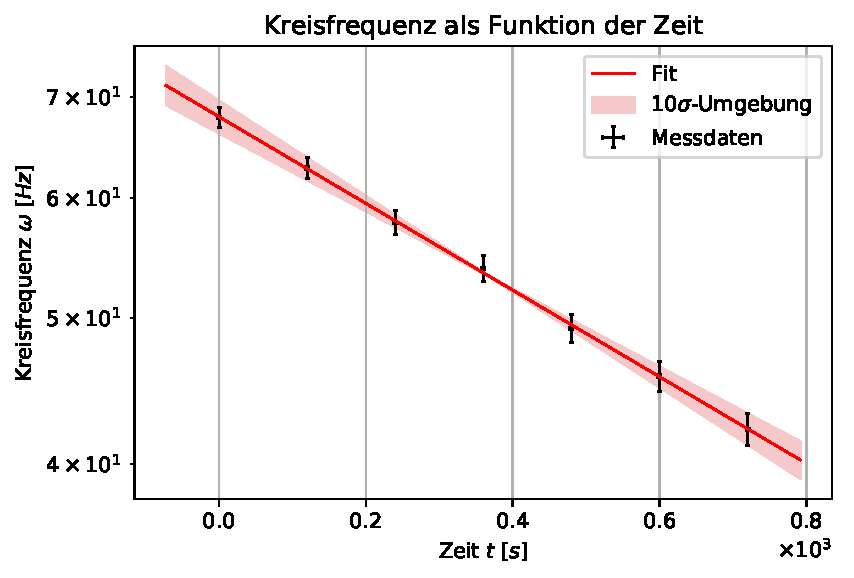
\includegraphics[width=0.8\textwidth]{213_Fig1.pdf}}{1}
  \end{annotate}
\caption{}
\label{fig:Fig1}
\end{figure}
\subsection{Auswertung}
Die gemessenen Wert für die Dämpfungskonstante \(k\) und Halbwertszeit \(T_{1/2}\) machen Sinn und passen zu unserem theoretischem Modell \eqref{eq:Fit1}:
\begin{align*}
k&=6.600(66)\times10^{-4}\: Hz\\
T_{1/2}&=1.050(11)\times10^{3}\:s
\end{align*}
Der jedoch geringe Wert \(\chi^{2}_{red}=4.5\times10^{-2}\) sagt uns, dass die bei der Messung geschätzten Messunsicherheiten zu groß abgeschätzt worden sind. D.h.  \(\Delta k\) und \(\Delta T_{1/2}\) sind größtenteils aus statistischen Unsicherheiten hervorgegangen, existierende systematische Fehler waren Größenordnungen kleiner und beeinträchtigten die Messung und das Ergebnis nicht signifikant. Nur durch genaueres bestimmen der statischen Messunsicherheiten oder mehr Messungen, können \(\Delta k\) und \(\Delta T_{1/2}\) verringert werden und gegebenenfalls systematische Fehler gefunden, analysiert und korrigiert werden.\\
Die Kreisfrequenz als Funktion der Zeit ist in Abbildung \ref{fig:Fig1} dargestellt.\\
\section{Bestimmung von \(I_{z}\) aus der Präzessionsfrequenz}
\subsection[Durchführung]{Durchführung\fnrefb}
Bei allen Messungen dieser Aufgabe wird der Kreisel zunächst bei senkrechter  Achse auf die gewünschte Geschwindigkeit gebracht. Anschließend wird die Achse durch Angreifen am Kugellager schräg gestellt und kurz vor der
gewählten Ablesemarke möglichst nutationsfrei losgelassen. Als Ablesemarke dient ein Messingstab in der Kreiselbasis.
\begin{enumerate}[label=(\alph*)]
\item Zuerst montieren wir die Farbscheibe auf den Stab und vergewissern uns,
dass der Kreisel kräftefrei ist. Im Abstand von \(l=20\: cm\) zur Kugelmitte wird ein Zusatzgewicht auf den Stab montiert. Die Drehgeschwindigkeit wird zuerst auf \(f_F \approx 500 \: min^{-1} \) eingestellt. Den Stab wird bei gleicher Drehgeschwindigkeit des Kreisels möglichst nutationsfrei unter drei verschiedenen
Winkeln des Stabs gegen die Vertikale losgelassen und die Zeit \(T_P\), in die Rotationsachse des Kreisels einen ganzen Umlauf vollzieht,  bestimmt.

\item Wir belasten den kräftefreien Kreisel mit folgenden Zusatzmassen:
\begin{itemize}
\item Ein Gewichtsstück bei \(l=20\: cm\) (*). 
\item Ein Gewichtsstück bei \(l=15\: cm\).
\item Zwei Gewichtsstücke bei \(l=20\: cm\).
\item Zwei Gewichtsstücke bei \(l=15\: cm\). 
\end{itemize}
Gemessen wird mit der Stoppuhr die
Präzessionsdauer \(T_P\) für jede Gewichtseinstellung bei jeweils vier verschiedene Frequenzen \(f_F\) im Bereich \(250 \:{min}^{-1} < f_F < 700\:{min}^{-1}\). Zur ersten Messreihe (*) können wir auch die Messdaten aus der vorherigen Aufgabe hinzufügen, da es genau die gleichen Messkriterien  (\(n=1\),\(l=20\: cm\))  erfüllt. Bbei jeder Masseneinstellung beginnen wir bei einer hohen
Frequenz und bremsen dann für die folgenden Messungen den Kreisel etwas ab. Für jede Messung notieren wir die Frequenz \(f_F\) und die Präzessionsdauer \(T_P\) .
\end{enumerate}

\subsection{Messergebnisse}
Messdaten wurden dem Versuchsprotokoll (22. Oktober, 2019) entnommen und in Tabelle \ref{tab:Tab2} übertragen.
\unboldmath
\begin{table}[htb]
\centering
\caption{Messung der  Präzessionsdauer}\label{tab:Tab2}
\begin{threeparttable}
\begin{tabular}{ccccc}
\toprule
Messreihe & Eigenfrequenz \boldmath\(f_F\)\unboldmath & Präzessionsdauer \boldmath\(T_P\)\unboldmath  &Abstand \boldmath\(l\)\unboldmath & Anzahl der Gewichte  \boldmath\(n\)\unboldmath \\
\(Aufgabe_{Nr.}\)&\([min^{-1}]\)&\([s]\)&\([cm]\)&\([1]\)\\
\midrule
\((a)\)&\(500\pm10\)&\(74.80\pm0.30\)&\(20.0\pm0.1\)&\(1\)\\
\(''\)&\(500\pm10\)&\(75.00\pm0.30\)&\(''\)&\(''\)\\
\(''\)&\(500\pm10\)&\(74.80\pm0.30\)&\(''\)&\(''\)\\
\midrule
\((b_1)\)(*)&\(298\pm10\)&\(47.90\pm0.30\)&\(20.0\pm0.1\)&\(1\)\\
\(''\)&\(404\pm10\)&\(64.00\pm0.30\)&\(''\)&\(''\)\\
\(''\)&\(501\pm10\)&\(78.50\pm0.30\)&\(''\)&\(''\)\\
\(''\)&\(602\pm10\)&\(92.51\pm0.30\)&\(''\)&\(''\)\\
\midrule
\((b_2)\)&\(297\pm10\)&\(61.46\pm0.30\)&\(15.0\pm0.1\)&\(1\)\\
\(''\)&\(407\pm10\)&\(85.31\pm0.30\)&\(''\)&\(''\)\\
\(''\)&\(495\pm10\)&\(101.56\pm0.30\)&\(''\)&\(''\)\\
\(''\)&\(601\pm10\)&\(122.67\pm0.30\)&\(''\)&\(''\)\\
\midrule
\((b_3)\)&\(599\pm10\)&\(44.76\pm0.30\)&\(20.0\pm0.1\)&\(2\)\\
\(''\)&\(502\pm10\)&\(38.28\pm0.30\)&\(''\)&\(''\)\\
\(''\)&\(403\pm10\)&\(30.72\pm0.30\)&\(''\)&\(''\)\\
\(''\)&\(301\pm10\)&\(23.04\pm0.30\)&\(''\)&\(''\)\\
\midrule
\((b_4)\)&\(603\pm10\)&\(61.06\pm0.30\)&\(15.0\pm0.1\)&\(2\)\\
\(''\)&\(499\pm10\)&\(50.67\pm0.30\)&\(''\)&\(''\)\\
\(''\)&\(300\pm10\)&\(32.23\pm0.30\)&\(''\)&\(''\)\\
\(''\)&\(298\pm10\)&\(31.06\pm0.30\)&\(''\)&\(''\)\\
\bottomrule
 \end{tabular}
\begin{tablenotes}
\raggedright
\item[1] \boldmath\(\Delta f_{F} \) grob abgeschätzt\unboldmath
\item[2] \boldmath\(\Delta T_{P} \) grob abgeschätzt als durchschnittliche menschliche  Reaktionszeit von 200 ms und Faktor \(\sqrt{2}\), weil zum Messen die Stoppuhr doppelt betätigt werden muss:  \(0.2\:s\times\sqrt{2}\approx0.3\:s = \Delta T_{P} \)\unboldmath
\item[(*)] Zu dieser Messreihe wird im weiteren Verlauf auch Messreihe (a) gezählt
\end{tablenotes}
\end{threeparttable}\end{table}
\boldmath
Die Masse eines einzelnen Gewichts beträgt
\[m_{G}=9.85(1)\:g\]
und die Erdbeschleunigung nähern wir mit
\[g=9.851(1)\:m\:s^{-2}\]
\subsection{Kurvenanpassung mit Python, Schritt 1}
\subsubsection{Source Code \& Input}
Wir drücken \(f_F\) über die entsprechende Kreisfrequenz \(\omega_{F}\) aus:
\begin{equation} \label{eq:omega_F}
	\omega_{F}=2\pi f_{F}
\end{equation} 
\begin{equation} \label{eq:Deltaomega_F}
	\Delta\omega_{F}=2\pi (\Delta f_{F})
\end{equation} 
Wir gehen davon aus, dass die Präzessionsdauer proportional zur Eigenkreisfrequenz zunimmt.
Daher ist unser funktionales Modell für die Ausgleichungsrechnung wie folgt:
\begin{equation} \label{eq:Fit2}
	\boxed{T_P = S \omega_{F}}
\end{equation} 
So sieht die Fortführung unserer Python-Implementierung aus:\\

Messwerte aus Tabelle \ref{tab:Tab2} in SI Einheiten (vorerst nicht nach Messreihen aufgeteilt):
\begin{lstlisting}
f_F = np.array([500,500,500,298,404,501,602,297,407,495, 601,599,502,403,301,603,499,300,298]) /60 ]
Fehler_f_F = np.full(f_F.size, 10) /60

T_P = np.array([74.80,75.00,75.39,47.90,64.00,78.50,92.51,61.46,85.31,101.56, 122.67,44.76,
                38.28,30.72,23.04,61.06,50.67,32.23,31.06]) 
Fehler_T_P = np.full(T_P.size, 0.30)

\end{lstlisting}

Berechnung der Eigenkreisfrequenz  \(\omega_F\) und \(\Delta\omega_F\) nach \eqref{eq:omega_F} bzw. \eqref{eq:Deltaomega_F}:\begin{lstlisting}
omega_F = 2*np.pi*f_F
Fehler_omega_F = 2*np.pi*Fehler_f_F
                  
\end{lstlisting}

 Fitfunktion \eqref{eq:Fit2} wird deklariert:\begin{lstlisting}
from scipy import odr

def fit_func(p, x):
    (s) = p 
    return s*x

model = odr.Model(fit_func)

\end{lstlisting}

darzustellende Daten werden übergeben (aufgeteilt auf die Messreihen \((a)+(b_1)\), \((b_2)\), \((b_3)\) und \((b_4)\)):\begin{lstlisting}
x_1 = omega_F[0:7]
y_1 = T_P[0:7]
delta_x_1 = Fehler_omega_F[0:7]
delta_y_1 = Fehler_T_P[0:7]

x_2 = omega_F[7:11]
y_2 = T_P[7:11]
delta_x_2 = Fehler_omega_F[7:11]
delta_y_2 = Fehler_T_P[7:11]

x_3 = omega_F[11:15]
y_3 = T_P[11:15]
delta_x_3 = Fehler_omega_F[11:15]
delta_y_3 = Fehler_T_P[11:15]

x_4 = omega_F[15:19]
y_4 = T_P[15:19]
delta_x_4 = Fehler_omega_F[15:19]
delta_y_4 = Fehler_T_P[15:19]

\end{lstlisting}

Startparameter für Ausgleichungsrechnung werden gesetzt, sodass Lösung konvergiert:\begin{lstlisting}
para0 = [1]

data_1 = odr.RealData(x_1, y_1, sx=delta_x_1, sy=delta_y_1)
odr_1 = odr.ODR(data_1, model, beta0=para0 )
out_1 = odr_1.run()

data_2 = odr.RealData(x_2, y_2, sx=delta_x_2, sy=delta_y_2)
odr_2 = odr.ODR(data_2, model, beta0=para0 )
out_2 = odr_2.run()

data_3 = odr.RealData(x_3, y_3, sx=delta_x_3, sy=delta_y_3)
odr_3 = odr.ODR(data_3, model, beta0=para0 )
out_3 = odr_3.run()

data_4 = odr.RealData(x_4, y_4, sx=delta_x_4, sy=delta_y_4)
odr_4 = odr.ODR(data_4, model, beta0=para0 )
out_4 = odr_4.run()

\end{lstlisting}

Endgültige Ausgleichungsparameter und ihre Kovarianzmatrix werden ausgelesen:\begin{lstlisting}
popt_1 = out_1.beta
perr_1 = out_1.sd_beta

popt_2 = out_2.beta
perr_2 = out_2.sd_beta

popt_3 = out_3.beta
perr_3 = out_3.sd_beta

popt_4 = out_4.beta
perr_4 = out_4.sd_beta

\end{lstlisting}

Angabe welche Sigma-Umgebung der Fitfunktion im Diagramm dargestellt werden soll:\begin{lstlisting}
nstd = 1

popt_top_1 = popt_1+nstd*perr_1
popt_bot_1 = popt_1-nstd*perr_1

popt_top_2 = popt_2+nstd*perr_2
popt_bot_2 = popt_2-nstd*perr_2

popt_top_3 = popt_3+nstd*perr_3
popt_bot_3 = popt_3-nstd*perr_3

popt_top_4 = popt_4+nstd*perr_4
popt_bot_4 = popt_4-nstd*perr_4

\end{lstlisting}

Plot-Umgebung wird angegeben:\begin{lstlisting}
x_fit_1 = np.linspace(min(x_1)-(max(x_1)-min(x_1))/10, max(x_1)+(max(x_1)-min(x_1))/10, 1000)
fit_1 = fit_func(popt_1, x_fit_1)
fit_top_1 = fit_func(popt_top_1, x_fit_1)
fit_bot_1 = fit_func(popt_bot_1, x_fit_1)

x_fit_2 = np.linspace(min(x_2)-(max(x_2)-min(x_2))/10, max(x_2)+(max(x_2)-min(x_2))/10, 1000)
fit_2 = fit_func(popt_2, x_fit_2)
fit_top_2 = fit_func(popt_top_2, x_fit_2)
fit_bot_2 = fit_func(popt_bot_2, x_fit_2)

x_fit_3 = np.linspace(min(x_3)-(max(x_3)-min(x_3))/10, max(x_3)+(max(x_3)-min(x_3))/10, 1000)
fit_3 = fit_func(popt_3, x_fit_3)
fit_top_3 = fit_func(popt_top_3, x_fit_3)
fit_bot_3 = fit_func(popt_bot_3, x_fit_3)

x_fit_4 = np.linspace(min(x_4)-(max(x_4)-min(x_4))/10, max(x_4)+(max(x_4)-min(x_4))/10, 1000)
fit_4 = fit_func(popt_4, x_fit_4)
fit_top_4 = fit_func(popt_top_4, x_fit_4)
fit_bot_4 = fit_func(popt_bot_4, x_fit_4)

\end{lstlisting}

Diagramm (Abb.\ref{fig:Fig2}) wird erstellt:\begin{lstlisting}
fig, ax = plt.subplots(1, figsize=[6.4 *1.5, 4.8])
plt.ticklabel_format(axis='both', style='sci', scilimits=(0,3), useMathText=True)
plt.errorbar(x_1, y_1, yerr=delta_y_1, xerr=delta_x_1, lw=1, ecolor='k', fmt='none', capsize=1, label='Messdaten 1')
plt.errorbar(x_2, y_2, yerr=delta_y_2, xerr=delta_x_2, lw=1, ecolor='k', fmt='none', capsize=1, label='Messdaten 2')
plt.errorbar(x_3, y_3, yerr=delta_y_3, xerr=delta_x_3, lw=1, ecolor='k', fmt='none', capsize=1, label='Messdaten 3')
plt.errorbar(x_4, y_4, yerr=delta_y_4, xerr=delta_x_4, lw=1, ecolor='k', fmt='none', capsize=1, label='Messdaten 4')
plt.title('Präzessionsdauer als Funktion der Eigenkreisfrequenz')
plt.grid(True)
plt.xlabel('Eigenkreisfrequenz '+r'${\omega_F}$'+' '+r'${[Hz]}$')
plt.ylabel('Präzessionsdauer '+r'${T_P}$'+' '+r'${[s]}$')
plt.plot(x_fit_1, fit_1, color='C3', lw=1, label='Fit  1')
plt.plot(x_fit_2, fit_2, color='C2', lw=1, label='Fit  2')
plt.plot(x_fit_3, fit_3, color='C0', lw=1, label='Fit  3')
plt.plot(x_fit_4, fit_4, color='C1', lw=1, label='Fit  4')
ax.fill_between(x_fit_1, fit_top_1, fit_bot_1, color='C3', alpha=.25, label=str(nstd)+r'$\sigma$'+'-Umgebung 1')
ax.fill_between(x_fit_2, fit_top_2, fit_bot_2, color='C2', alpha=.25, label=str(nstd)+r'$\sigma$'+'-Umgebung 2')
ax.fill_between(x_fit_3, fit_top_3, fit_bot_3, color='C0', alpha=.25, label=str(nstd)+r'$\sigma$'+'-Umgebung 3')
ax.fill_between(x_fit_4, fit_top_4, fit_bot_4, color='C1', alpha=.25, label=str(nstd)+r'$\sigma$'+'-Umgebung 4')
box = ax.get_position()
ax.set_position([box.x0, box.y0, box.width * 0.8, box.height])
ax.legend(loc='center left', bbox_to_anchor=(1, 0.5))

plt.savefig('figures/213_Fig2.pdf', format='pdf', bbox_inches='tight')

\end{lstlisting}

Auslesen der Messergebnisse:\begin{lstlisting}
S_1 = popt_1[0]
Fehler_S_1 = perr_1[0]
S_2 = popt_2[0]
Fehler_S_2 = perr_2[0]
S_3 = popt_3[0]
Fehler_S_3 = perr_3[0]
S_4 = popt_4[0]
Fehler_S_4 = perr_4[0]

\end{lstlisting}

Der Chi-Quadrat-Test wird durchgeführt unter Berücksichtigung von \(\Delta \omega_F\) und \(\Delta T_P\). D.h.~es wird jeweils der senkrechte/orthogonale Abstand der Messwerte zur Fitfunktion (Abb.\ref{fig:chi}) berechnet und normiert\fnrefa.

\begin{lstlisting}
dof_1 = x_1.size-popt.size
chisquare_1 = out_1.sum_square
chisquare_red_1 = chisquare_1/dof_1
prob_1 = round(1-chi2.cdf(chisquare_1,dof_1),2)*100

dof_2 = x_2.size-popt.size
chisquare_2 = out_2.sum_square
chisquare_red_2 = chisquare_2/dof_2
prob_2 = round(1-chi2.cdf(chisquare_2,dof_2),2)*100

dof_3 = x_3.size-popt.size
chisquare_3 = out_3.sum_square
chisquare_red_3 = chisquare_3/dof_3
prob_3 = round(1-chi2.cdf(chisquare_3,dof_3),2)*100

dof_4 = x_4.size-popt.size
chisquare_4 = out_4.sum_square
chisquare_red_4 = chisquare_4/dof_4
prob_4 = round(1-chi2.cdf(chisquare_4,dof_4),2)*100

\end{lstlisting}

Ausgabe der Messergebnisse wird erstellt:\begin{lstlisting}
print('Steigungen: ')
print('S_1 [s^2] =', format_e(S_1), ' +- ', format_e(Fehler_S_1))
print('Chi-Quadrat =', chisquare_1)
print('Freiheitsgrade =', dof_1)
print('Chi-Quadrat reduziert =', chisquare_red_1)
print('Wahrscheinlichkeit ein größeres oder gleiches Chi-Quadrat zu erhalten =', prob_1, '%')
print('\n')
print('S_2 [s^2] =', format_e(S_2), ' +- ', format_e(Fehler_S_2))
print('Chi-Quadrat =', chisquare_2)
print('Freiheitsgrade =', dof_2)
print('Chi-Quadrat reduziert =', chisquare_red_2)
print('Wahrscheinlichkeit ein größeres oder gleiches Chi-Quadrat zu erhalten =', prob_2, '%')
print('\n')
print('S_3 [s^2] =', format_e(S_3), ' +- ', format_e(Fehler_S_3))
print('Chi-Quadrat =', chisquare_3)
print('Freiheitsgrade =', dof_3)
print('Chi-Quadrat reduziert =', chisquare_red_3)
print('Wahrscheinlichkeit ein größeres oder gleiches Chi-Quadrat zu erhalten =', prob_3, '%')
print('\n')
print('S_4 [s^2] =', format_e(S_4), ' +- ', format_e(Fehler_S_4))
print('Chi-Quadrat =', chisquare_4)
print('Freiheitsgrade =', dof_4)
print('Chi-Quadrat reduziert =', chisquare_red_4)
print('Wahrscheinlichkeit ein größeres oder gleiches Chi-Quadrat zu erhalten =', prob_4, '%')
print('\n')
\end{lstlisting}

\subsubsection{Output}
\begin{lstlisting}
Steigungen: 
S_1 [s^2] = 1.465235e+00  +-  1.366893e-02
Chi-Quadrat = 8.120624052429571
Freiheitsgrade = 5
Chi-Quadrat reduziert = 1.6241248104859143
Wahrscheinlichkeit ein größeres oder gleiches Chi-Quadrat zu erhalten = 15.0 %

S_2 [s^2] = 1.965064e+00  +-  1.134583e-02
Chi-Quadrat = 0.8421813756024409
Freiheitsgrade = 2
Chi-Quadrat reduziert = 0.42109068780122044
Wahrscheinlichkeit ein größeres oder gleiches Chi-Quadrat zu erhalten = 66.0 %

S_3 [s^2] = 7.224199e-01  +-  4.304101e-03
Chi-Quadrat = 0.7948108139557275
Freiheitsgrade = 2
Chi-Quadrat reduziert = 0.39740540697786375
Wahrscheinlichkeit ein größeres oder gleiches Chi-Quadrat zu erhalten = 67.0 %

S_4 [s^2] = 9.780491e-01  +-  1.114486e-02
Chi-Quadrat = 2.8383188936144617
Freiheitsgrade = 2
Chi-Quadrat reduziert = 1.4191594468072308
Wahrscheinlichkeit ein größeres oder gleiches Chi-Quadrat zu erhalten = 24.0 %

\end{lstlisting}
Wir erfahren also sofort, dass
\begin{align*}
S_1&=1.465(14)\: s^2\\
S_2&=1.965(11)\: s^2\\
S_3&=7.224(43)\times10^{-1}\: s^2\\
S_4&=9.78(11)\times10^{-1}\: s^2
\end{align*}
und als Ergebnis auf unseren Anpassungstests:
\begin{align*}
\chi^{2}_{red,1}&=1.6\\
\chi^{2}_{red,2}&=4.2\times10^{-1}\\
\chi^{2}_{red,3}&=4.0\times10^{-1}\\
\chi^{2}_{red,4}&=1.4
\end{align*}
Die Wahrscheinlichkeiten ein größeres oder gleiches Chi-Quadrat zu erhalten sind jeweils
\begin{align*}
P_1\approx  15.0 \%\\
P_2\approx  66.0 \%\\
P_3\approx  67.0 \%\\
P_4\approx  24.0 \%
\end{align*}
und wir erhalten das Diagramm in Abb.\ref{fig:Fig2}.
\begin{figure}[htb]
  \centering
  \begin{annotate}{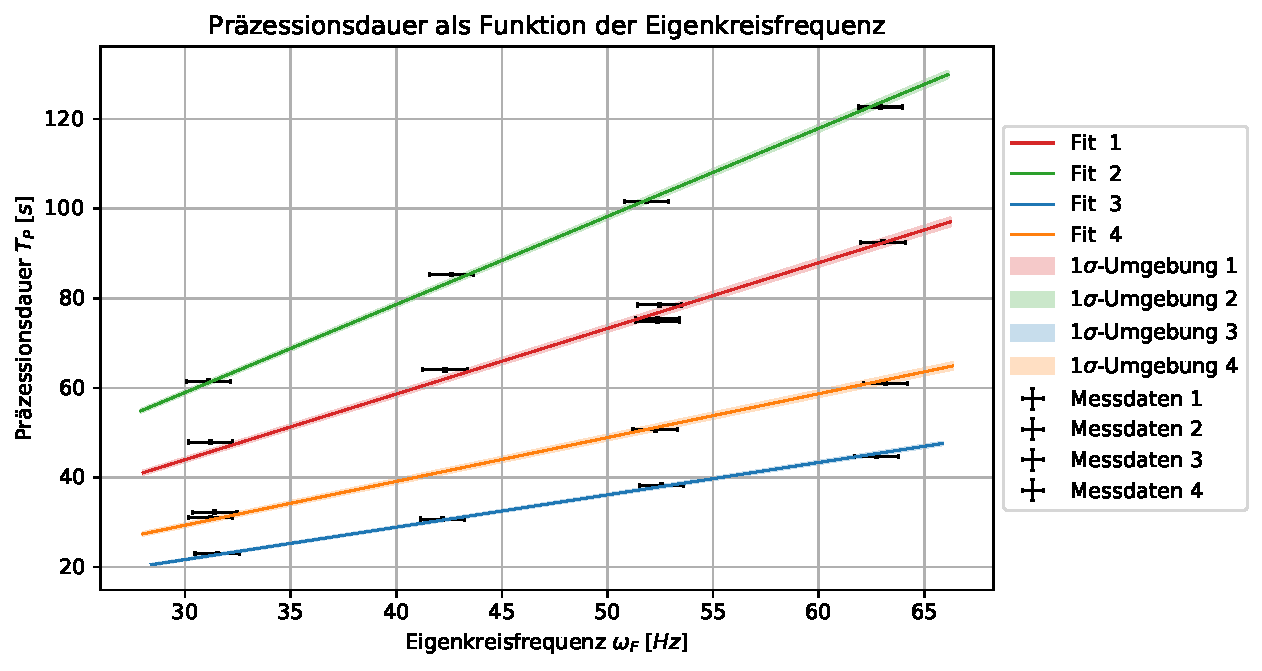
\includegraphics[width=0.8\textwidth]{213_Fig2.pdf}}{1}
  \end{annotate}
\caption{}
\label{fig:Fig2}
\end{figure}
\subsection{Kurvenanpassung mit Python, Schritt 2}
\subsubsection{Source Code \& Input}
Wir gehen davon aus, dass das Trägheitsmoment konstant ist.
Daher ist unser funktionales Modell für die Ausgleichungsrechnung wie folgt:
\begin{equation} \label{eq:Fit3}
	\boxed{I_z = konst.}
\end{equation} 
Für diesen Schritt, benutzen wir die Angaben aus "Versuchsaufbau, Literaturwerte \& Vorbereitung" 
\begin{align*}
g&=9.80984(2)\:m\:s^2\\
m_G&=9,85(1)\: g
\end{align*}
und die Messergebnisse aus Schritt 1 um das Trägheitsmoment um die Figurenachse zu berechnen:
\begin{equation} \label{eq:m}
	m={m_{G}} \times n
\end{equation} 
\begin{equation} \label{eq:Deltam}
	\Delta m= {\Delta m_{G}}\times \sqrt{n}
\end{equation} 
\begin{equation} \label{eq:I_z}
	I_z = \frac{m g l S}{2 \pi}
\end{equation} 
\begin{equation} \label{eq:DeltaI_z}
	\Delta I_z = |I_z| \sqrt{{\left( \frac{\Delta m}{m} \right)}^2+{\left( \frac{\Delta g}{g}\right)}^2+{\left(\frac{\Delta l}{l}\right)}^2+{\left( \frac{\Delta S}{S}\right )}^2}
\end{equation} 
So sieht die Fortführung unserer Python-Implementierung aus:\\

Messwerte der Steigung S aus Schritt 1 in SI Einheiten:
\begin{lstlisting}
S = np.array([S_1,S_2,S_3,S_4])
Fehler_S = np.array([Fehler_S_1,Fehler_S_2,Fehler_S_3,Fehler_S_4])

\end{lstlisting}

Messwerte aus Tabelle \ref{tab:Tab2} in SI Einheiten:\begin{lstlisting}
l = np.array([20,15,20,15]) /1e2
Fehler_l = np.full(l.size, 0.1) /1e2

n =  np.array([1,1,2,2])

\end{lstlisting}

Angaben aus "Versuchsaufbau, Literaturwerte \& Vorbereitung"  in SI Einheiten:\begin{lstlisting}
m_G = 9.85 /1e3 
Fehler_m_G = 0.01 /1e3

g = 9.80984
Fehler_g = 0.00002

\end{lstlisting}

Berechnung der Masse  \(m\) und \(\Delta m\) nach \eqref{eq:m} bzw. \eqref{eq:Deltam}:\begin{lstlisting}
m = n*m_G
Fehler_m = np.sqrt(n)* Fehler_m_G

\end{lstlisting}

Berechnung des Trägheitsmoments \(I_z\) und \(\Delta I_z\) nach \eqref{eq:I_z} bzw. \eqref{eq:DeltaI_z}:\begin{lstlisting}
I_z = m*g*l*S/(2*np.pi)
Fehler_I_z = abs(I_z)*np.sqrt((Fehler_m/m)**2+(Fehler_g/g)**2+(Fehler_l/l)**2+(Fehler_S/S)**2)

\end{lstlisting}

Fitfunktion \eqref{eq:Fit3} wird deklariert:\begin{lstlisting}
from scipy import odr

def fit_func(p, x):
    (c) = p
    return x*0+c

model = odr.Model(fit_func)

\end{lstlisting}

darzustellende Daten werden übergeben:\begin{lstlisting}
x = S
y = I_z
delta_x = Fehler_S
delta_y = Fehler_I_z

\end{lstlisting}

Startparameter für Ausgleichungsrechnung werden gesetzt, sodass Lösung konvergiert:\begin{lstlisting}
para0 = [0]

data = odr.RealData(x, y, sx=delta_x, sy=delta_y)
odr = odr.ODR(data, model, beta0=para0 )
out = odr.run()

\end{lstlisting}

Endgültige Ausgleichungsparameter und ihre Kovarianzmatrix werden ausgelesen:\begin{lstlisting}
popt = out.beta
perr = out.sd_beta

\end{lstlisting}

Angabe welche Sigma-Umgebung der Fitfunktion im Diagramm dargestellt werden soll:\begin{lstlisting}
nstd = 1

popt_top = popt+nstd*perr
popt_bot = popt-nstd*perr

\end{lstlisting}

Plot-Umgebung wird angegeben:\begin{lstlisting}
x_fit = np.linspace(min(x)-(max(x)-min(x))/10, max(x)+(max(x)-min(x))/10, 1000)
fit = fit_func(popt, x_fit)
fit_top = fit_func(popt_top, x_fit)
fit_bot = fit_func(popt_bot, x_fit)

\end{lstlisting}

Diagramm (Abb.\ref{fig:Fig3}) wird erstellt:\begin{lstlisting}
fig, ax = plt.subplots(1)
plt.ticklabel_format(axis='both', style='sci', scilimits=(0,3), useMathText=True)
plt.errorbar(x, y, yerr=delta_y, xerr=delta_x, lw=1, ecolor='k', fmt='none', capsize=1, label='Messdaten')
plt.title('Trägheitsmoment')
plt.grid(True)
plt.xlabel('Steigung '+r'${S}$'+' '+r'${[s^2]}$')
plt.ylabel('Trägheitsmoment '+r'${I_z}$' + ' '+r'${[s]}$')
plt.plot(x_fit, fit, color='r', lw=1, label='Fit')
ax.fill_between(x_fit, fit_top, fit_bot, color='C3', alpha=.25, label=str(nstd)+r'$\sigma$'+'-Umgebung')
plt.legend(loc='best')

plt.savefig('figures/213_Fig3.pdf', format='pdf', bbox_inches='tight')

\end{lstlisting}

Auslesen der Messergebnisse:\begin{lstlisting}
I_z = popt[0]
Fehler_I_z = perr[0]

\end{lstlisting}

Der Chi-Quadrat-Test wird durchgeführt unter Berücksichtigung von \(\Delta S\) und \(\Delta I_z\). D.h.~es wird jeweils der senkrechte/orthogonale Abstand der Messwerte zur Fitfunktion (Abb.\ref{fig:chi}) berechnet und normiert\fnrefa .
 Die Summe der normierten Abstandsquadrate, der \unboldmath\( \chi^{2}\)-Wert, wird  reduziert.\boldmath

\begin{lstlisting}
dof = x.size-popt.size
chisquare = out.sum_square
chisquare_red = chisquare/dof
prob = round(1-chi2.cdf(chisquare,dof),2)*100

\end{lstlisting}

Ausgabe der Messergebnisse wird erstellt:\begin{lstlisting}
print('Trägheitsmoment: ')
print('I_z [kg * m^2] =', format_e(I_z), ' +- ', format_e(Fehler_I_z))
print('Chi-Quadrat =', chisquare)
print('Freiheitsgrade =', dof)
print('Chi-Quadrat reduziert =', chisquare_red)
print('Wahrscheinlichkeit ein größeres oder gleiches Chi-Quadrat zu erhalten =', prob, '%')

\end{lstlisting}

\subsubsection{Output}

\begin{lstlisting}
Trägheitsmoment: 
I_z [kg * m^2] = 4.490859e-03  +-  2.207146e-05
Chi-Quadrat = 3.162438468024628
Freiheitsgrade = 3
Chi-Quadrat reduziert = 1.0541461560082093
Wahrscheinlichkeit ein größeres oder gleiches Chi-Quadrat zu erhalten = 37.0 %

\end{lstlisting}
Wir erfahren also sofort, dass
\[I_z =4.491(22)\times10^{-3}\: kg\: m^2\]
und als Ergebnis auf unseren Anpassungstest:
\[\chi^{2}_{red}=1.1\]
Die Wahrscheinlichkeit ein größeres oder gleiches Chi-Quadrat zu erhalten ist
 \[P \approx 37.0 \%\]
und wir erhalten das Diagramm in Abb.\ref{fig:Fig3}.
\begin{figure}[htb]
  \centering
  \begin{annotate}{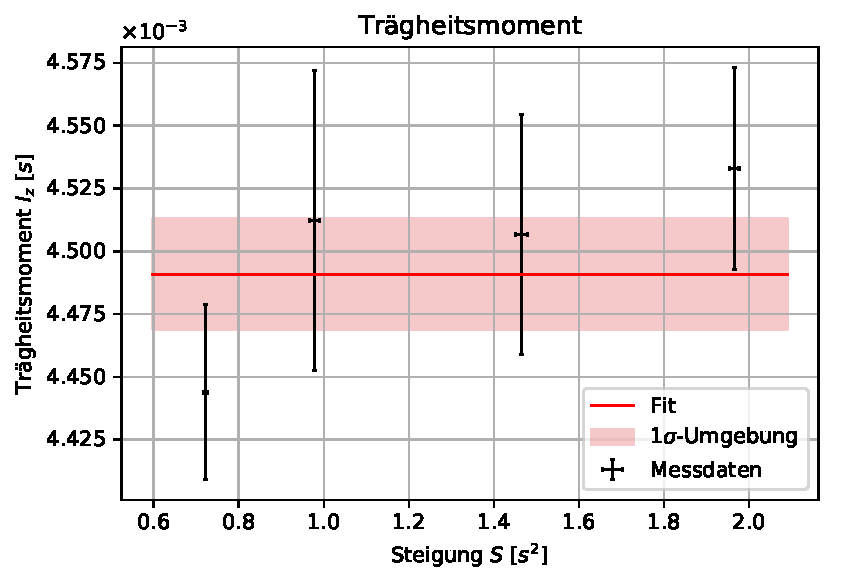
\includegraphics[width=0.8\textwidth]{213_Fig3.pdf}}{1}
  \end{annotate}
\caption{}
\label{fig:Fig3}
\end{figure}
\subsection{Auswertung}
\begin{enumerate}[label=(\alph*)]
\item Wie erwartet hat die Messreihe (a) Zeiten geliefert die nicht signifikant von einander abweichen (siehe Tab. \ref{tab:Tab2a}). Alle 3 Werte liegen paarweise jeweils in der 1-Sigma-Umgebung von einander. Das stimmt mit unserem theoretischen Modell überein, dass die Präzessionsdauer, bei konstanter Eigenfrequenz \(f_F\) und Drehmoment\(M\) bzw. Gewichtskonfiguration \(\{ n, l\}\), sich nicht ändert. Auch in diesem Versuch überwiegen die statistischen Messunsicherheiten jegliche systematischen Fehler. Nur durch viel genaueres bestimmen der statischen Messunsicherheiten oder mehr Messungen, können dieses systematische Fehler gefunden, analysiert und gegebenenfalls korrigiert werden.
\unboldmath
\begin{table}[htb]
\centering
\caption{Messung der  Präzessionsdauer}\label{tab:Tab2a}
\begin{threeparttable}
\begin{tabular}{ccccc}
\toprule
Messreihe & Eigenfrequenz \boldmath\(f_F\)\unboldmath & Präzessionsdauer \boldmath\(T_P\)\unboldmath  &Abstand \boldmath\(l\)\unboldmath & Anzahl der Gewichte  \boldmath\(n\)\unboldmath \\
\(Aufgabe_{Nr.}\)&\([min^{-1}]\)&\([s]\)&\([cm]\)&\([1]\)\\
\midrule
\((a)\)&\(500\pm10\)&\(74.80\pm0.30\)&\(20.0\pm0.1\)&\(1\)\\
\(''\)&\(500\pm10\)&\(75.00\pm0.30\)&\(''\)&\(''\)\\
\(''\)&\(500\pm10\)&\(74.80\pm0.30\)&\(''\)&\(''\)\\
\bottomrule
 \end{tabular}
\begin{tablenotes}
\raggedright
\item[1] \boldmath\(\Delta f_{F} \) grob abgeschätzt\unboldmath
\item[2] \boldmath\(\Delta T_{P} \) grob abgeschätzt als durchschnittliche menschliche  Reaktionszeit von 200 ms und Faktor \(\sqrt{2}\), weil zum Messen die Stoppuhr doppelt betätigt werden muss:  \(0.2\:s\times\sqrt{2}\approx0.3\:s = \Delta T_{P} \)\unboldmath
\end{tablenotes}
\end{threeparttable}\end{table}
\boldmath
\item
Die gemessenen Werte für die 4 Steigungen \(S_i\) und \(I_z\)machen Sinn und passen zu unserem theoretischen Modellen \eqref{eq:Fit2} und \eqref{eq:Fit3} :
\begin{align*}
S_1&=1.465(14)\: s^2\\
S_2&=1.965(11)\: s^2\\
S_3&=7.224(43)\times10^{-1}\: s^2\\
S_4&=9.78(11)\times10^{-1}\: s^2\\
I_z &=4.491(22)\times10^{-3}\: kg\: m^2
\end{align*}
Die Präzessionsdauern als Funktionen der Eigenkreisfrequenz aus jeder Messreihe sind in Abbildung \ref{fig:Fig2} dargestellt.\\
Das resultierenden Messwerte für das Trägheitsmomente aus den einzelnen Messreihen und ihr Mittelwert sind in Abbildung \ref{fig:Fig3} dargestellt.\\
Die Wahrscheinlichkeiten ein größeres oder gleiches Chi-Quadrat zu erhalten
\begin{align*}
P_1\approx  15.0 \%\\
P_2\approx  66.0 \%\\
P_3\approx  67.0 \%\\
P_4\approx  24.0 \%\\
 P \approx 37.0 \%
\end{align*} sind auch alle in Ordnung. Weder waren unsere Abschätzungen für die Messunsicherheiten signifikant zu groß, weder sind wir auf signifikante systematische Fehler getroffen, die eine Korrektur von unseren theoretischen Modellen verlangen würden. Letzteres kann sich aber wie immer bei zunehmender Beseitigung statistischer Fehler und weitere Analyse ändern.



\end{enumerate}
\section{Bestimmung von \(I_{x}\) aus der Größe und der Richtung der Umlaufschwindigkeit}
\subsection[Durchführung]{Durchführung\fnrefb}
Wir überprüfen, ob der Kreisel kräftefrei ist und versetzen anschließend
den Kreisel bei senkrechter Achse mit Hilfe des Motors in Rotation. Nach dem
Anwerfen wird durch einen leichten seitlichen Stoß auf die Achse, der Kreisel in
Nutation versetzt.
\begin{enumerate}[label=(\alph*)]
\item Die Umlaufrichtung der momentanen Drehachse wird mit
Hilfe der Farbscheibe bestimmt. Dafür beachten wir die Reihenfolge der Farben im einfarbigen Punkt.

\item Mit der Stoppuhr messen wir für 10 Frequenzen im Bereich \(300 \:{min}^{-1} < f_F < 600\:{min}^{-1}\) jeweils die Zeit \(T_{10}\) für 10 Umläufe der momentanen Drehachse um die Figurenachse. Die Frequenz des Farbwechsels \(\Omega\) der Sektorscheib entspricht genau der
Umlaufsgeschwindigkeit \(\Omega\) der momentanen Drehachse um die Figurenachse des Kreisels.
\end{enumerate}
\subsection{Messergebnisse}
\begin{enumerate}[label=(\alph*)]
\item In unserem Versuch rotierte der Kreisel von oben betrachtet gegen den Uhrzeigersinn. Die Farben im einfarbigem Punkt folgten der zeitlichen Reihenfolge "Gelb, Rot, Grün, Gelb...", was auf unserer Scheibe mit den Sektoren auch der Reihenfolge gegen den Uhrzeigersinn entspricht. D.h. bei unserem Kreisel zeigen \(\vec{\Omega}\) und \(\vec{\omega}_F\) in ungefähr die gleiche Richtung \((\vec{\Omega} \vec{\omega}_F > 0)\). Sie haben also das gleiche Vorzeichen in der Gleichung 
\begin{equation} \label{eq:sign}
	\Omega= \frac{{I_x}-{I_z}}{I_x}{\omega_F}
\end{equation} 
die, die Geometrie der Nutationsbewegung für symmetrische, kräftefreie Kreisel beschreibt.

\item Messdaten wurden dem Versuchsprotokoll (22. Oktober, 2019) entnommen und in Tabelle \ref{tab:Tab3} übertragen.
\unboldmath
\begin{table}[htb]
\centering
\caption{Messung der Periode vom Farbwechsel}\label{tab:Tab3}
\begin{threeparttable}
\begin{tabular}{ccccc}
\toprule
Eigenfrequenz \boldmath\(f_F\)\unboldmath & Dauer von 10 Perioden \boldmath\(T_{10}\)\unboldmath\\
\([min^{-1}]\)&\([s]\)\\
\midrule
\(485\pm10\)&\(22.37\pm0.30\)\\
\(360\pm10\)&\(29.90\pm0.30\)\\
\(511\pm10\)&\(21.37\pm0.30\)\\
\(397\pm10\)&\(28.01\pm0.30\)\\
\(460\pm10\)&\(23.29\pm0.30\)\\
\(415\pm10\)&\(26.48\pm0.30\)\\
\(560\pm10\)&\(19.89\pm0.30\)\\
\(510\pm10\)&\(20.53\pm0.30\)\\
\(460\pm10\)&\(23.17\pm0.30\)\\
\(400\pm10\)&\(26.42\pm0.30\)\\
\bottomrule
 \end{tabular}
\begin{tablenotes}
\raggedright
\item[1] \boldmath\(\Delta f_{F} \) grob abgeschätzt\unboldmath
\item[2] \boldmath\(\Delta T_{10} \) grob abgeschätzt als durchschnittliche menschliche  Reaktionszeit von 200 ms und Faktor \(\sqrt{2}\), weil zum Messen die Stoppuhr doppelt betätigt werden muss:  \(0.2\:s\times\sqrt{2}\approx0.3\:s = \Delta T_{P} \)\unboldmath
\end{tablenotes}
\end{threeparttable}\end{table}
\boldmath
\end{enumerate}
\subsection{Kurvenanpassung mit Python}
\subsubsection{Source Code \& Input}
Wir können sofort folgende Zusammenhänge schließen:
\begin{equation} \label{eq:T_Farbe}
	T_{Farbe} = T_{10}/10
\end{equation} 
\begin{equation} \label{eq:DeltaT_Farbe}
	\Delta T_{Farbe} = (\Delta T_{10})/10
\end{equation} 

\begin{equation} \label{eq:absOmega}
	|\Omega| = \frac{2 \pi}{T_{Farbe}}
\end{equation} 
Wie sich in \eqref{eq:sign} herausstellt, zeigen \(\vec{\Omega}\) und \(\vec{\omega}_F\) in die gleiche Richtung, deswegen gilt:
\begin{equation} \label{eq:absOmega}
	\Omega= \frac{2 \pi}{T_{Farbe}} 
\end{equation} 
\begin{equation} \label{eq:DeltaOmega}
	\Delta \Omega = |\Omega|{\left( \frac{\Delta T_{Farbe}}{T_{Farbe}} \right)}
\end{equation} 
Wir gehen davon aus, dass die Umlaufsgeschwindigkeit \(\Omega\) proportional zur Eigenkreisfrequenz zunimmt.
Daher ist unser funktionales Modell für die Ausgleichungsrechnung wie folgt:
\begin{equation} \label{eq:Fit4}
	\boxed{\Omega = S_{Farbe} \omega_{F}}
\end{equation} 
Aus \eqref{eq:sign} und \eqref{eq:Fit4} folgt außerdem:
\begin{equation} \label{eq:I_x1}
	I_{x,1} = \frac{I_z}{1-{S_{Farbe}}}
\end{equation} 
\begin{equation*} \label{eq:DeltaI_x1}
	\Delta I_{x,1}  = |I_{x,1} | \sqrt{\left(\frac{\Delta I_z}{I_z}\right)^2+\left(\frac{\Delta (1-S_{Farbe})}{1-{S_{Farbe}}}\right)^2} 
\end{equation*} 
\begin{equation} \label{eq:DeltaI_x1}
	= |I_{x,1} | \sqrt{\left(\frac{\Delta I_z}{I_z}\right)^2+\left(\frac{\Delta S_{Farbe}}{1-{S_{Farbe}}}\right)^2}
\end{equation} 
So sieht die Fortführung unserer Python-Implementierung aus:\\

Messwerte aus Tabelle \ref{tab:Tab3} in SI Einheiten:
\begin{lstlisting}
f_F = np.array([485,360,511,397,460,415,560,510,460,400]) /60
Fehler_f_F = np.full(f_F.size, 10) /60

T_10 = np.array([22.37,29.90,21.37,28.01,23.29,26.48,19.89,20.53,23.17,26.42]) 
Fehler_T_10 = np.full(T_Farbe.size, 0.30)

\end{lstlisting}

Berechnung der Periode vom Farbwechsel \(T_{Farbe}\) und \(\Delta T_{Farbe}\) nach \eqref{eq:T_Farbe} bzw. \eqref{eq:DeltaT_Farbe}:\begin{lstlisting}
T_Farbe = T_10/10
Fehler_T_Farbe = Fehler_T_10 /10

\end{lstlisting}

Berechnung der Eigenkreisfrequenz  \(\omega_F\) und \(\Delta\omega_F\) nach \eqref{eq:omega_F} bzw. \eqref{eq:Deltaomega_F}:\begin{lstlisting}
omega_F = 2*np.pi*f_F 
Fehler_omega_F = 2*np.pi*Fehler_f_F

Omega = 2*np.pi/T_Farbe 
Fehler_Omega = 2*np.pi*Omega*Fehler_T_Farbe/T_Farbe

\end{lstlisting}

Fitfunktion \eqref{eq:Fit4} wird deklariert:\begin{lstlisting}
from scipy import odr

def fit_func(p, x):
    (s) = p
    return x*s

model = odr.Model(fit_func)

\end{lstlisting}

darzustellende Daten werden übergeben:\begin{lstlisting}
x = omega_F
y = Omega
delta_x = Fehler_omega_F
delta_y = Fehler_Omega

\end{lstlisting}

Startparameter für Ausgleichungsrechnung werden gesetzt, sodass Lösung konvergiert:\begin{lstlisting}
para0 = [1]

data = odr.RealData(x, y, sx=delta_x, sy=delta_y)
odr = odr.ODR(data, model, beta0=para0 )
out = odr.run()

\end{lstlisting}

Endgültige Ausgleichungsparameter und ihre Kovarianzmatrix werden ausgelesen:\begin{lstlisting}
popt = out.beta
perr = out.sd_beta

\end{lstlisting}

Angabe welche Sigma-Umgebung der Fitfunktion im Diagramm dargestellt werden soll:\begin{lstlisting}
nstd = 1 

popt_top = popt+nstd*perr
popt_bot = popt-nstd*perr

\end{lstlisting}

Plot-Umgebung wird angegeben:\begin{lstlisting}
x_fit = np.linspace(min(x)-(max(x)-min(x))/10, max(x)+(max(x)-min(x))/10, 1000)
fit = fit_func(popt, x_fit)
fit_top = fit_func(popt_top, x_fit)
fit_bot = fit_func(popt_bot, x_fit)

\end{lstlisting}

Diagramm (Abb.\ref{fig:Fig4}) wird erstellt:\begin{lstlisting}
fig, ax = plt.subplots(1)
plt.errorbar(x, y, yerr=delta_y, xerr=delta_x, lw=1, ecolor='k', fmt='none', capsize=1, label='Messdaten')
plt.title('Winkelgeschwindigkeit der Drehachse als Funktion der Eigenkreisfrequenz')
plt.grid(True)
plt.xlabel('Eigenkreisfrequenz '+r'${\omega_F}$'+' '+r'${[Hz]}$')
plt.ylabel('Winkelgeschwindigkeit '+r'${\Omega}$'+' '+r'${[Hz]}$')
plt.plot(x_fit, fit, color='C3', lw=1, label='Fit')
ax.fill_between(x_fit, fit_top, fit_bot, color='r', alpha=.25, label=str(nstd)+r'$\sigma$'+'-Umgebung')
plt.legend(loc='best')

plt.savefig('figures/213_Fig4.pdf', format='pdf', bbox_inches='tight')

\end{lstlisting}

Auslesen der Messergebnisse:\begin{lstlisting}
S_Farbe = popt[0]
Fehler_S_Farbe = perr[0]

\end{lstlisting}

Berechnung des Trägheitsmoments \(I_{x,1}\) und \(\Delta I_{x,1}\) nach \eqref{eq:I_x1} bzw. \eqref{eq:DeltaI_x1}:\begin{lstlisting}
I_x_1 = I_z/(1-S_Farbe)
Fehler_I_x_1 = abs(I_x_1)*np.sqrt((Fehler_I_z/I_z)**2+(Fehler_S_Farbe/(1-S_Farbe))**2)

\end{lstlisting}
Der Chi-Quadrat-
Test wird durchgeführt unter Berücksichtigung von \(\Delta \omega_F\) und \(\Delta \Omega\). D.h.~es wird jeweils der senkrechte/orthogonale Abstand der Messwerte zur Fitfunktion (Abb.\ref{fig:chi}) berechnet und normiert\fnrefa.

\begin{lstlisting}
dof = x.size-popt.size
chisquare = out.sum_square
chisquare_red = chisquare/dof
prob = round(1-chi2.cdf(chisquare,dof),2)*100

\end{lstlisting}

Ausgabe der Messergebnisse wird erstellt:\begin{lstlisting}
print('Steigung:')
print('S_Farbe =', format_e(S_Farbe), ' +- ', format_e(Fehler_S_Farbe))
print('Chi-Quadrat =', chisquare)
print('Freiheitsgrade =', dof)
print('Chi-Quadrat reduziert =', chisquare_red)
print('Wahrscheinlichkeit ein größeres oder gleiches Chi-Quadrat zu erhalten =', prob, '%')
print('\n')
print('1.Messmethode:')
print('I_x_1 [kg * m^2] =', format_e(I_x_1), ' +- ', format_e(Fehler_I_x_1))
\end{lstlisting}

\subsubsection{Output}
\begin{lstlisting}
Steigung:
S_Farbe = 5.54362e-02  +-  3.58525e-04
Chi-Quadrat = 1.8131534915537362
Freiheitsgrade = 9
Chi-Quadrat reduziert = 0.20146149906152624
Wahrscheinlichkeit ein größeres oder gleiches Chi-Quadrat zu erhalten = 99.0 %

1.Messmethode:
I_x_1 [kg * m^2] = 4.754426e-03  +-  2.343641e-05
\end{lstlisting}
Wir erfahren also sofort, dass
\begin{align*}
S_{Farbe}&=5.544(36)\times10^{-2}\\
I_{x,1}&=4.754(23)\times10^{-3}\:kg\: m^2
\end{align*}
und als Ergebnis auf unseren Anpassungstest:
\[\chi^{2}_{red}=2.0\times10^{-1}\]
Die Wahrscheinlichkeit ein größeres oder gleiches Chi-Quadrat zu erhalten ist
 \[P\approx  99.0 \%\]
und wir erhalten das Diagramm in Abb.\ref{fig:Fig4}.
\begin{figure}[htb]
  \centering
  \begin{annotate}{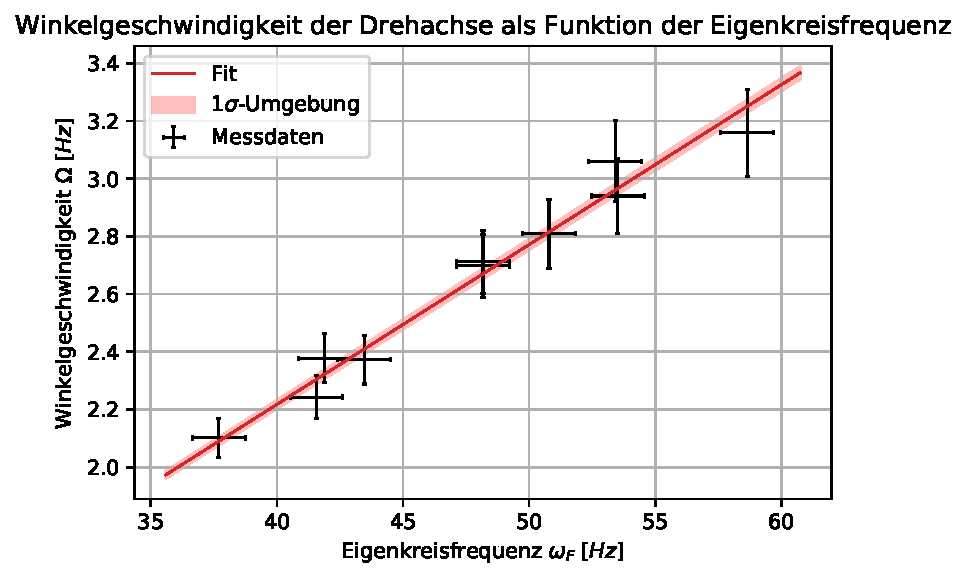
\includegraphics[width=0.8\textwidth]{213_Fig4.pdf}}{1}
  \end{annotate}
\caption{}
\label{fig:Fig4}
\end{figure}
\subsection{Auswertung}
\begin{enumerate}[label=(\alph*)]
\item Unsere Beobachtungen lassen eindeutig darauf schließen, dass in unserem theoretischem Modell \eqref{eq:sign} \(\Omega\) und \(\omega_F\) das gleiche Vorzeichen haben. Deswegen folgt auch \[(\Delta I = {I_x}-{I_z}>0 )\iff({I_x}>{I_z} )\]Das wird sich ein zweites Mal bestätigen lassen können, wenn wir \(I_z\) aus dem vorherigen Versuchsteil mit dem Wert für \(I_{x,2}\)  aus der 2. Messmethode im nächsten Versuchsteil vergleichen.


\item Die Winkelgeschwindigkeit der Drehachse als Funktion der Eigenkreisfrequenz ist in Abbildung \ref{fig:Fig4} dargestellt. Die Wahrscheinlichkeit ein größeres oder gleiches Chi-Quadrat zu erhalten
 \(P\approx  99.0 \%\) ist ein Zeichen dafür, dass wahrscheinlich wieder Messunsicherheiten größer abgeschätzt wurden als sie es sind. Deswegen können wir wieder nur schlecht systematische Fehler in unserem theoretischem Modell feststellen ohne mehr Messdaten zu erheben oder mit anderen Messungen zu vergleichen.
\begin{align*}
S_{Farbe}&=5.544(36)\times10^{-2}\\
I_{x,1}&=4.754(23))\times10^{-3}\:kg\: m^2
\end{align*}
\end{enumerate}

\section{Bestimmung von \(I_{x}\) aus der Nutationsfrequenz}
\subsection[Durchführung]{Durchführung\fnrefb}
Wir versetzenden kräftefreien Kreisel durch vorsichtiges Anschlagen an
die Achse in Nutation. Damit die Näherung 
\begin{equation} \label{eq:approx}
	\omega_N = \frac{I_z}{I_x}\omega_F
\end{equation}
gilt, sollte die Öffnung des Nutationskegels an der Spitze des Stabes nur \(1-2\:cm\) betragen. Bei unserer Durchführung war dieser Wert 
eher größer \(\approx 2-3\:cm\), weil sich bei Versuchen einen kleineren Nutationskegel zu erhalten, diese so klein ausfielen,dass die Messung mit dem Stroboskop sich als unpraktisch erwies.  Nun bestimmt man 10 Wertepaare von \(f_N\) und \(f_F\) . Wir sind dabei
folgendermaßen vogegangen: eher langsamere Messung der Nutationsfrequenz mit dem Stroboskop zu Beginn und erst bei der Festlegung von \(f_N\) wird \(f_F\)  mit Hilfe des optischen Drehzahlmessers.

\subsection{Messergebnisse}
Messdaten wurden dem Versuchsprotokoll (22. Oktober, 2019) entnommen und in Tabelle \ref{tab:Tab4} übertragen.
\unboldmath
\begin{table}[htb]
\centering
\caption{Messung der Nutationsfrequenz}\label{tab:Tab4}
\begin{threeparttable}
\begin{tabular}{cc}
\toprule
Nutationsfrequenz \boldmath\(f_N\)\unboldmath & Drehfrequenz \boldmath\(f_F\)\unboldmath \\
\([min^{-1}]\)&\([min^{-1}]\)\\
\midrule
\(655\pm5\)&\(693\pm10\)\\
\(585\pm5\)&\(601\pm10\)\\
\(435\pm5\)&\(444\pm10\)\\
\(525\pm5\)&\(574\pm10\)\\
\(255\pm5\)&\(488\pm10\)\\
\(780\pm5\)&\(637\pm10\)\\
\(695\pm5\)&\(737\pm10\)\\
\(685\pm5\)&\(722\pm10\)\\
\(395\pm5\)&\(394\pm10\)\\
\(600\pm5\)&\(629\pm10\)\\
  \bottomrule
 \end{tabular}
\begin{tablenotes}
\raggedright
\item[1] \boldmath\(\Delta f_F \) grob abgeschätzt\unboldmath
\item[2] \boldmath\(\Delta f_N \) abgeschätzt als halbe Skaleneinteilung am Stroboskop\unboldmath
\end{tablenotes}
\end{threeparttable}\end{table}
\boldmath

\subsection{Kurvenanpassung mit Python}
\subsubsection{Source Code \& Input}
Wir drücken \(f_N\) über die entsprechende Kreisfrequenz \(\omega_{N}\) aus:
\begin{equation} \label{eq:omega_N}
	\omega_{N}=2\pi f_{N}
\end{equation} 
\begin{equation} \label{eq:Deltaomega_N}
	\Delta\omega_{N}=2\pi (\Delta f_{N})
\end{equation} 
Wir gehen davon aus, dass die Präzessionsdauer proportional zur Eigenkreisfrequenz zunimmt.
Daher ist unser funktionales Modell für die Ausgleichungsrechnung wie folgt:
\begin{equation} \label{eq:Fit5}
	\boxed{\omega_{N} = {S_N} \omega_{F}}
\end{equation} 
So sieht die Fortführung unserer Python-Implementierung aus:\\
Messwerte aus Tabelle \ref{tab:Tab4} in SI Einheiten:
\begin{lstlisting}
f_F = np.array([693,601,444,574,488,837,737,722,394,629]) /6
Fehler_f_F = np.full(f_F.size, 10) /60

f_N = np.array([655,585,435,525,455,780,695,685,395,600]) /60 
Fehler_f_N = np.full(T_Farbe.size, 5) /60

\end{lstlisting}

Berechnung der Eigenkreisfrequenz  \(\omega_F\) und \(\Delta\omega_F\) nach \eqref{eq:omega_F} bzw. \eqref{eq:Deltaomega_F}:\begin{lstlisting}
omega_F = 2*np.pi*f_F 
Fehler_omega_F = 2*np.pi*Fehler_f_F

\end{lstlisting}

Berechnung der Nutationskreisfrequenz  \(\omega_N\) und \(\Delta\omega_N\) nach \eqref{eq:omega_N} bzw. \eqref{eq:Deltaomega_N}:\begin{lstlisting}
omega_N = 2*np.pi*f_N
Fehler_omega_N = 2*np.pi*Fehler_f_N

\end{lstlisting}

Fitfunktion \eqref{eq:Fit5} wird deklariert:\begin{lstlisting}
from scipy import odr

def fit_func(p, x):
    (s) = p
    return x*s

model = odr.Model(fit_func)

\end{lstlisting}

darzustellende Daten werden übergeben:\begin{lstlisting}
x = omega_F
y = omega_N
delta_x = Fehler_omega_F
delta_y = Fehler_omega_N

\end{lstlisting}

Startparameter für Ausgleichungsrechnung werden gesetzt, sodass Lösung konvergiert:\begin{lstlisting}
para0 = [1]

data = odr.RealData(x, y, sx=delta_x, sy=delta_y)
odr = odr.ODR(data, model, beta0=para0 )
out = odr.run()


\end{lstlisting}

Auslesen der Messergebnisse:\begin{lstlisting}
popt = out.beta
perr = out.sd_beta

\end{lstlisting}

Angabe welche Sigma-Umgebung der Fitfunktion im Diagramm dargestellt werden soll:\begin{lstlisting}
nstd = 2

popt_top = popt+nstd*perr
popt_bot = popt-nstd*perr

\end{lstlisting}

Plot-Umgebung wird angegeben:\begin{lstlisting}
x_fit = np.linspace(min(x)-(max(x)-min(x))/10, max(x)+(max(x)-min(x))/10, 1000)
fit = fit_func(popt, x_fit)
fit_top = fit_func(popt_top, x_fit)
fit_bot = fit_func(popt_bot, x_fit)

\end{lstlisting}

Diagramm (Abb.\ref{fig:Fig5}) wird erstellt:\begin{lstlisting}
fig, ax = plt.subplots(1)
plt.errorbar(x, y, yerr=delta_y, xerr=delta_x, lw=1, ecolor='k', fmt='none', capsize=1, label='Messdaten')
plt.title('Nutationsfrequenz als Funktion der Eigenfrequenz')
plt.grid(True)
plt.xlabel('Eigenkreisfrequenz '+r'${\omega_F}$'+' '+r'${[Hz]}$')
plt.ylabel('Nutationskreisfrequenz '+r'${\omega_N}$'+' '+r'${[Hz]}$')
plt.plot(x_fit, fit, color='C3', lw=1, label='Fit')
ax.fill_between(x_fit, fit_top, fit_bot, color='C3', alpha=.25, label=str(nstd)+r'$\sigma$'+'-Umgebung')
plt.legend(loc='best')

plt.savefig('figures/213_Fig5.pdf', format='pdf', bbox_inches='tight')

\end{lstlisting}

Endgültige Ausgleichungsparameter und ihre Kovarianzmatrix werden ausgelesen:\begin{lstlisting}
S_N = popt[0]
Fehler_S_N = perr[0]

I_x_2 = I_z/S_N
Fehler_I_x_2 = abs(I_x_2)*np.sqrt((Fehler_I_z/I_z)**2+(Fehler_S_N/S_N)**2)

\end{lstlisting}

Der Chi-Quadrat-Test wird durchgeführt unter Berücksichtigung von \(\Delta \omega_F\) und \(\Delta \omega_N\). D.h.~es wird jeweils der senkrechte/orthogonale Abstand der Messwerte zur Fitfunktion (Abb.\ref{fig:chi}) berechnet und normiert\fnrefa.

\begin{lstlisting}
dof = x.size-popt.size
chisquare = out.sum_square
chisquare_red = chisquare/dof
prob = round(1-chi2.cdf(chisquare,dof),2)*100

\end{lstlisting}

Ausgabe der Messergebnisse wird erstellt:\begin{lstlisting}
print('Steigung: ')
print('S_N =', format_e(S_N), ' +- ', format_e(Fehler_S_N))
print('Chi-Quadrat =', chisquare)
print('Freiheitsgrade =', dof)
print('Chi-Quadrat reduziert =', chisquare_red)
print('Wahrscheinlichkeit ein größeres oder gleiches Chi-Quadrat zu erhalten =', prob, '%')
print('\n')
print('2.Messmethode: ')
print('I_x [kg * m^2] =', format_e(I_x_2), ' +- ', format_e(Fehler_I_x_2))
\end{lstlisting}

\subsubsection{Output}
\begin{lstlisting}
Steigung: 
S_N = 9.474419e-01  +-  6.580497e-03
Chi-Quadrat = 13.315446247417999
Freiheitsgrade = 9
Chi-Quadrat reduziert = 1.4794940274908888
Wahrscheinlichkeit ein größeres oder gleiches Chi-Quadrat zu erhalten = 15.0 %

2.Messmethode: 
I_x [kg * m^2] = 4.739983e-03  +-  4.033036e-05
\end{lstlisting}
Wir erfahren also sofort, dass
\begin{align*}
S_{N}&=9.474(66)\times10^{-1}\\
I_{x,2}&=4.739(40)\times10^{-3}\:kg\: m^2
\end{align*}
und als Ergebnis auf unseren Anpassungstest:
\[\chi^{2}_{red}=1.5\]
Die Wahrscheinlichkeit ein größeres oder gleiches Chi-Quadrat zu erhalten ist
 \[P\approx  15.0 \%\]
und wir erhalten das Diagramm in Abb.\ref{fig:Fig4}.
\begin{figure}[htb]
  \centering
  \begin{annotate}{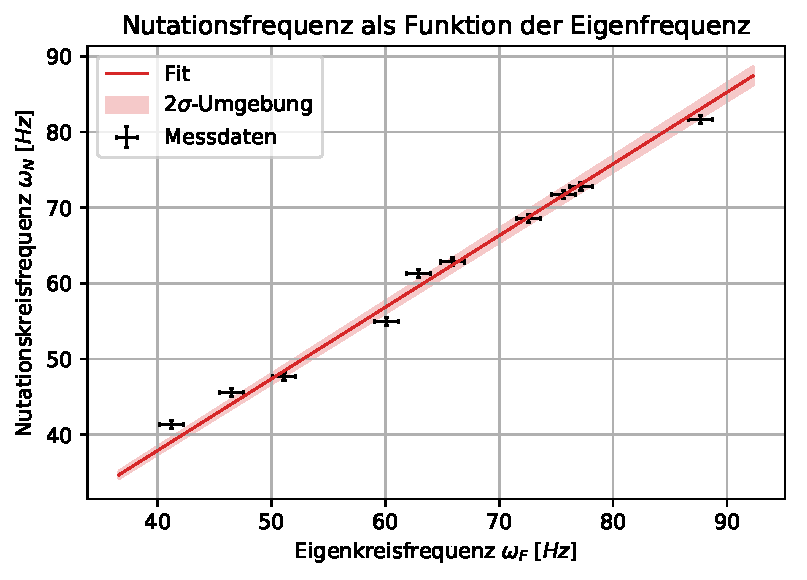
\includegraphics[width=0.8\textwidth]{213_Fig5.pdf}}{1}
  \end{annotate}
\caption{}
\label{fig:Fig5}
\end{figure}
\subsection{Auswertung}
\begin{align*}
S_{N}&=9.474(66)\times10^{-1}\\
I_{x,2}&=4.739(40))\times10^{-3}\:kg\: m^2
\end{align*}
Die 'Nutationsfrequenz als Funktion der Eigenfrequenz ist in Abbildung \ref{fig:Fig5} dargestellt.
Die Wahrscheinlichkeit ein größeres oder gleiches Chi-Quadrat \(P\approx  15.0 \%\) ist in Ordnung. Unsere Abschätzungen für die Messunsicherheiten waren also nicht signifikant zu groß. Weil wir in \eqref{eq:approx} eine Näherung durchgeführt habe, haben wir garantiert systematische Fehler, aber für die relativ kleinen Nutationswinkel sollten diese im Größenordnungen von einigen Prozent liegen. In diesem Größenbereich halten sich auch unsere statistischen Messfehler auf:
	\[\frac{\Delta I_{x,2}}{I_{x,2}} = 0.84\%\]
D.h. es ist eher unwahrscheinlich das der systematische und somit gesammte Fehler von \( I_{x,2}\) 5\% überschreitet. Wenn aber der systematische Fehler signifikanter ist als der statistische, müsste unser Messwert signifikant von \( I_{x,1}\) aus der 1. Messmethode abweichen.

\section{Fazit}
Die gemessenen Wert für die Dämpfungskonstante \(k\) und Halbwertszeit \(T_{1/2}\) sind:
\begin{align*}
k&=6.600(66)\times10^{-4}\: Hz\\
T_{1/2}&=1.050(11)\times10^{3}\:s
\end{align*}
und für die jeweiligen Trägheitsmomente:
\begin{align*}
I_z &=4.491(22)\times10^{-3}\: kg\: m^2\\
I_{x,1}&=4.754(23)\times10^{-3}\:kg\: m^2\\
I_{x,2}&=4.739(40)\times10^{-3}\:kg\: m^2\\
\end{align*}
Wenn wir uns diese Werte anschauen. Merken wir als erstes, dass  \( I_{x,1}\) und  \( I_{x,2}\) jeweils in der 1-Sigma-Umgebung von einander liegen und somit sich nicht signifikant unterscheiden. Daraus können wir folgende Aussagen schließen: 
\begin{itemize}
\item Die Näherung \eqref{eq:approx}  war gut genug und innerhalb unserer statistischen Messfehler von \( I_{x,2}\) .
\item
\(( I_{x,2}> I_{z})\) mit einer statistischen Signifikanz von \[\frac{ I_{x,2}- I_{z}}{\sqrt{(\Delta  I_{x,2})^2+(\Delta  I_{z})^2}}= 5.4\]
also mehr als 5-Sigma Gewissheit \(\approx1-\left(3\times 10^{-8}\right)=99,999997\%\). Das bestätigt also nochmal unsere Bestimmung 
der Richtung von \(\vec{\Omega}\) gegenüber \(\vec{\omega}_F\).
\end{itemize}
\unboldmath
\end{document}
